\footnotesize
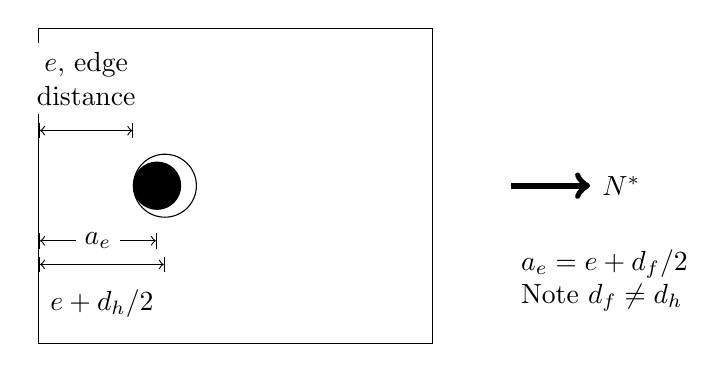
\begin{tikzpicture}
\draw(-1,-2)rectangle(4,2);
\draw(.6,0)circle(4mm);
\draw[fill=black](.5,0)circle(3mm);
\draw[|<->|](-1,.7)--(.2,.7)node[midway,fill=white,align=center,above=2mm]{$e$, edge\\distance};
\draw[|<->|](-1,-.7)--(.5,-.7)node[midway,fill=white]{$a_e$};
\draw[|<->|](-1,-1)--(.6,-1)node[midway,below=2mm]{$e+d_h/2$};
\draw[->,line width=.8mm](5,0)--++(1,0)node[right]{$N^*$};
\node[align=left,anchor=west]at(5,-1.2){$a_e=e+d_f/2$\\Note $d_f\neq{}d_h$};
\end{tikzpicture}